\documentclass[
	article,
	12pt,
	oneside,
	a4paper,
	english,
	brazil, % ultimo idioma é o principal do documento
	sumario=tradicional
]{abntex2}

% Pacotes fundamentais
\usepackage{times}
\usepackage[T1]{fontenc}
\usepackage[utf8]{inputenc}
\usepackage{indentfirst}
\usepackage{color}
\usepackage{graphicx}
\usepackage{amsmath}
\usepackage{gensymb}
\usepackage{lscape}
\usepackage{pdflscape}
\usepackage[table,xcdraw]{xcolor}
\usepackage{float}
\usepackage{microtype}
\usepackage{multirow}
\usepackage[normalem]{ulem}
\usepackage{rotating}
\usepackage{booktabs}
\usepackage[alf,abnt-etal-cite=3,abnt-etal-list=0]{abntex2cite}
\usepackage{hyperref}
\usepackage{tabularx} % For tabularx environment
\usepackage{booktabs} % For \toprule, \midrule, and \bottomrule
\usepackage{caption} % For \captionsetup
\usepackage{makecell}
\newcommand{\theforeigntitle}[1]{\def\@theforeigntitle{#1}}

% Configurações de aparência do PDF final
\definecolor{blue}{RGB}{41,5,195}
\hypersetup{
	pdftitle={Trabalho final de Econometria III - Replicação do artigo "Political systems, regime memory, and economic freedom"},
	pdfauthor={Bruno Francisco Schaden},
	pdfsubject={Modelo de artigo científico com abnTeX2},
	pdfcreator={LaTeX with abnTeX2},
	pdfkeywords={abnt}{latex}{abntex}{abntex2}{artigo científico},
	colorlinks=true,
	linkcolor=blue,
	citecolor=blue,
	filecolor=magenta,
	urlcolor=blue,
	bookmarksdepth=4
}

% Configurações de margens
\setlrmarginsandblock{3cm}{2cm}{*}
\setulmarginsandblock{3cm}{2cm}{*}
\checkandfixthelayout

% Espaçamentos entre linhas e parágrafos
\setlength{\parindent}{1.5cm}
\setlength{\parskip}{0.2cm}
\OnehalfSpacing

% Informações de dados para CAPA e FOLHA DE ROSTO
\titulo{Trabalho de Crescimento e Desenvolvimento Econômico - O Papel das Instituições e da Governança no Desenvolvimento Econômico sob a Perspectiva Schumpeteriana}
\autor{Bruno Francisco Schaden \and Yasmin Metzler}
\local{Florianópolis}
\data{2024}

\begin{document}

\frenchspacing

% ELEMENTOS PRÉ-TEXTUAIS
\maketitle
\selectlanguage{english}

% Resumo em inglês
	\begin{resumoumacoluna}
	\noindent
	This paper investigates the impact of institutions and governance on long-term economic development from a Schumpeterian perspective. The focus is on analyzing how the quality of political and economic institutions influences growth, especially in developing countries. Based on the theory of creative destruction, the paper explores how business dynamics and innovation are affected by institutional factors, observing the effects of political connections and the regulatory environment on innovation and economic performance. The data analyzed include information on companies, politicians and economic indicators from several countries, seeking to correlate institutional variables with innovation capacity and business dynamism. The analysis reveals that strong institutions promote innovation and sustained growth, while institutional fragility perpetuates inefficiencies and inequalities.
	
	\textbf{Keywords:} institutions, governance, creative destruction, economic growth, innovation, Schumpeterian perspective.
	
	\textbf{JEL Classification:} O10, O43, P16, L26, D72.

	For more details, visit: \url{https://github.com/Schadenlord/crescimento-e-desenvolvimento}

	\end{resumoumacoluna}

\newpage

\selectlanguage{brazil}
% Resumo em português
\renewcommand{\resumoname}{Resumo}
\begin{resumoumacoluna}
\begin{otherlanguage*}{brazil}
    \noindent 
    Este trabalho investiga o impacto das instituições e da governança no desenvolvimento econômico de longo prazo, sob a perspectiva schumpeteriana. O foco reside na análise de como a qualidade das instituições políticas e econômicas influencia o crescimento, especialmente em países em desenvolvimento. Partindo da teoria da destruição criativa, explora-se como a dinâmica empresarial e a inovação são afetadas por fatores institucionais, observando os efeitos das conexões políticas e do ambiente regulatório sobre a inovação e o desempenho econômico. Os dados analisados incluem informações sobre empresas, políticos e indicadores econômicos de diversos países, buscando correlacionar as variáveis institucionais com a capacidade de inovação e o dinamismo empresarial. A análise revela que instituições sólidas promovem a inovação e o crescimento sustentado, enquanto a fragilidade institucional perpetua ineficiências e desigualdades.
    
    \textbf{Palavras-chave}: instituições, governança, destruição criativa, crescimento econômico, inovação, perspectiva schumpeteriana.
    
    \textbf{Classificação JEL:} O10, O43, P16, L26, D72.

	   Para mais detalhes, acesse: \url{https://github.com/Schadenlord/crescimento-e-desenvolvimento}

 \end{otherlanguage*}  
\end{resumoumacoluna}

\newpage


% ELEMENTOS TEXTUAIS
\textual


%\chapter{Introdução}


\section{Do Artigo Científico de Replicação}

O estudo de \cite{https://doi.org/10.1111/coep.12635} explora como sistemas políticos e a memória de regimes anteriores influenciam a liberdade econômica atual. A liberdade econômica é um conceito crítico que afeta o desenvolvimento econômico e social dos países. Este trabalho objetiva replicar os métodos e resultados de \cite{https://doi.org/10.1111/coep.12635} para confirmar a robustez das suas conclusões.

A motivação para esta replicação reside na importância de verificar a reprodutibilidade das pesquisas acadêmicas. Estudos replicados com sucesso reforçam a validade das teorias propostas e aumentam a confiança na literatura científica existente. A abordagem metodológica e os dados utilizados são detalhados nas seções subsequentes.


\subsection{Fonte dos Dados}
Os dados utilizados nesta replicação são provenientes das mesmas fontes mencionadas por \cite{https://doi.org/10.1111/coep.12635}. Utilizamos o dataset replicação composto de liberdade econômica do \cite{fraser2022} e variáveis políticas do \cite{polity2022}. Estes conjuntos de dados fornecem uma cobertura ampla e detalhada de indicadores econômicos e políticos ao longo do tempo.

Adicionalmente, também é incorporado no dataset dados demográficos e econômicos do Banco Mundial para controlar variáveis que possam influenciar a liberdade econômica. Estes dados permitem uma análise comparativa robusta entre diferentes países e regimes ao longo das últimas décadas.

\subsection{Memória de Regime}
A metodologia replicada segue os passos descritos por \cite{https://doi.org/10.1111/coep.12635} somente mudando o softwere de análise de Stata para Python. Utilizamos modelos de regressão linear múltipla para analisar a relação entre sistemas políticos, memória de regime e liberdade econômica. A variável dependente é o índice de liberdade econômica, enquanto as variáveis independentes incluem indicadores políticos e demográficos.

Para capturar os efeitos das mudanças institucionais lentas associadas à mudança de regime, utilizamos duas variáveis para construir nossa medida de memória de regime. Durable é uma variável de contagem que registra o tempo desde a mudança de regime mais recente. Para registrar um efeito na memória de regime, a pontuação máxima de durable para um determinado regime deve ser maior que zero. Polity2 controla o tipo de regime e varia de -10 a 10, com uma pontuação mais baixa indicando um regime mais autocrático e uma pontuação maior indicando um regime mais democrático.

Nossa medida de memória de regime de um país é melhor descrita como uma média ponderada das pontuações de polity2 pelo regime em que os pesos são determinados pela pontuação de durable de cada regime. A construção ampla é descrita da seguinte forma:

\[
\text{RegimeMemory}_{it} = \frac{\sum_{r=0}^{R} \left( w_{(t-1)r} \cdot \text{Polity2}_{(t-1-k)r} \right)}{\sum_{r=0}^{R} w_{(t-1)r}}
\]

onde $i$ e $t$ são índices para país e ano, respectivamente, e $r$ é o índice para o regime. Todas as referências temporais no lado direito são defasadas de modo que a memória de regime não é influenciada diretamente pelas pontuações contemporâneas de polity e durable — ela é destinada a representar puramente a memória dos regimes passados. O subscrito $k$ indexa o número de anos desde o término do regime anterior. Os pesos dos regimes são atribuídos com um valor inicial de um no primeiro ano de existência do regime. A influência desse regime, e portanto seu peso, é assumida como crescente a uma taxa de desconto constante (2,5\% e 12,5\% para os resultados principais apresentados aqui) a cada ano adicional em que o regime está em vigor. Uma vez que um regime termina, o peso atribuído à contribuição desse regime para a memória de regime começa a diminuir na mesma taxa de desconto. Nosso período de amostra para nossa análise de regressão começa em 1970; no entanto, a medida de memória de regime para um determinado país inclui a influência descontada de todos os regimes passados incluídos no conjunto de dados Polity IV.

\begin{figure}[h!]
    \centering
    \caption{Variável de memória de regime para Chile e França entre 1970 e 2015, utilizando taxas de desconto de 2,5\% e 12,5\%, assim como a medida de cálculo alternativa.}
    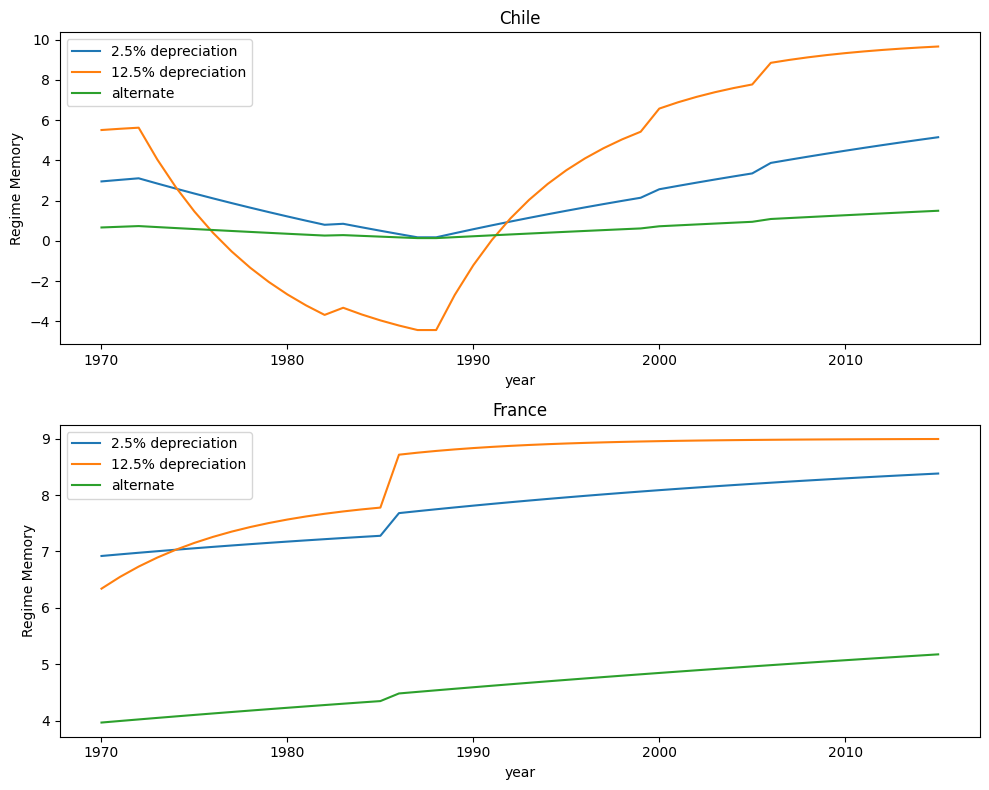
\includegraphics[width=0.8\textwidth]{Textuais/chile.png}
    \fonte{Replicação - Elaborado pelos autores.}
\end{figure}

\subsection{Metodologia Empírica}

A análise de regressão realizada utiliza o modelo de efeitos fixos para examinar a relação entre memória de regime e liberdade econômica. Este modelo permite controlar variáveis não observadas que são constantes ao longo do tempo, mas variam entre os países. A especificação do modelo é dada pela seguinte equação:

\begin{equation}
    \text{EFW}_{it} = \beta_1 \text{RegimeMemory}_{it} + \mathbf{X}_{it-1} \boldsymbol{\delta} + \Phi_t + \epsilon_{it} \quad 
\end{equation}

onde $i$ representa o índice de país e $t$ representa o índice de ano. Para explicar como a memória de regime afeta a liberdade econômica de um país, utilizamos o índice de Liberdade Econômica do Mundo (EFW) do projeto Economic Freedom of the World como nossa medida de liberdade econômica \cite{gwartney2022}. O índice varia de 0 a 10, com pontuações mais baixas denotando menos liberdade econômica e pontuações mais altas denotando mais liberdade.


\section{Resultados}

\subsection{Descrição dos Dados}
As estatísticas descritivas das variáveis foram reproduzidas quase perfeitamente, como mostrado na Tabela \ref{tab:tabela_descritiva}. A diferença encontrada nos números é de ordem de $10^{-2}$, o que é aceitável dada a natureza dos cálculos. A seguir, apresentamos uma breve descrição das variáveis utilizadas na análise:

\begin{itemize}
    \item \textbf{Memória de regime}: Medida que reflete a influência de regimes passados na liberdade econômica atual.
    \item \textbf{Net ODA as \% of GDP}: Ajuda externa líquida como percentual do PIB.
    \item \textbf{Resource rent as \% of GDP}: Renda de recursos como percentual do PIB.
    \item \textbf{ln(GDP per capita)}: Logaritmo do PIB per capita.
    \item \textbf{GDP Growth}: Crescimento do PIB.
    \item \textbf{War Dummy}: Variável indicativa de guerra.
    \item \textbf{Christian Dummy}: Variável indicativa de predominância cristã.
    \item \textbf{British legal origin}: Origem do sistema legal britânico.
    \item \textbf{French legal origin}: Origem do sistema legal francês.
    \item \textbf{Coup d'état}: Variável indicativa de golpes de estado.
    \item \textbf{Gini coefficient}: Coeficiente de Gini.
\end{itemize}

\begin{table}[htbp]
    \centering
    \renewcommand{\arraystretch}{1.1}
    \captionsetup{font=small}
    \caption{Tabela 2 do Artigo Original - Estatísticas Descritivas.}
    \label{tab:tabela_descritiva}
    \small % Ajusta o tamanho da fonte para 10 pontos
    \begin{tabularx}{\textwidth}{l*{8}{>{\raggedleft\arraybackslash}X}}
        \toprule
        \textbf{Variável} & \textbf{N} & \textbf{Média} & \textbf{Desv. Padrão} & \textbf{Mín.} & \textbf{25\%} & \textbf{50\%} & \textbf{75\%} & \textbf{Máx.} \\
        \midrule
        EFW index interpolated & 4697 & 6.14 & 1.30 & 2.37 & 5.18 & 6.20 & 7.18 & 8.85 \\
        EFW index not interpolated & 2534 & 6.53 & 1.16 & 2.37 & 5.75 & 6.65 & 7.44 & 8.85 \\
        2.5\% discount & 4697 & 0.38 & 6.05 & -10.0 & -4.93 & -0.54 & 6.00 & 10.0 \\
        5\% discount & 4697 & 1.01 & 6.34 & -10.0 & -4.84 & 0.79 & 7.00 & 10.0 \\
        7.5\% discount & 4697 & 1.43 & 6.51 & -10.0 & -4.72 & 2.01 & 7.90 & 10.0 \\
        10\% discount & 4697 & 1.73 & 6.64 & -10.0 & -4.65 & 3.03 & 8.03 & 10.0 \\
        12.5\% discount & 4697 & 1.95 & 6.73 & -10.0 & -4.59 & 3.70 & 8.61 & 10.0 \\
        15\% discount & 4697 & 2.10 & 6.79 & -10.0 & -4.63 & 4.00 & 8.89 & 10.0 \\
        Alternative & 4697 & 0.27 & 6.20 & -10.0 & -4.93 & 0.69 & 4.30 & 10.0 \\
        Net ODA as \% of GDP & 4697 & 3.28 & 5.59 & -0.40 & 0.00 & 0.69 & 3.07 & 81.43 \\
        Resource rent as \% of GDP & 4697 & 7.05 & 9.75 & 0.00 & 0.00 & 3.07 & 9.21 & 79.74 \\
        Real GDP per capita & 4697 & 11224.56 & 16503.12 & 157.10 & 1262.87 & 3731.68 & 14263.96 & 114047.91 \\
        GDP growth & 4697 & 3.67 & 4.94 & -50.25 & -4.93 & 0.79 & 7.00 & 39.49 \\
        War Dummy & 4697 & 0.09 & 0.28 & 0 & 0 & 0 & 0 & 1 \\
        Christian Dummy & 4697 & 0.63 & 0.48 & 0 & 0 & 1 & 1 & 1 \\
        UK legal origin & 4697 & 0.30 & 0.46 & 0 & 0 & 0 & 1 & 1 \\
        French legal origin & 4697 & 0.56 & 0.50 & 0 & 0 & 1 & 1 & 1 \\
        Coup d'etats & 4477 & 0.04 & 0.21 & 0 & 0 & 0 & 0 & 1 \\
        Gini & 3530 & 39.07 & 8.84 & 20.30 & 32.40 & 39.60 & 45.07 & 65.40 \\
        \bottomrule
    \end{tabularx}
    \fonte{Elaborado pelos autores.}
\end{table}


\subsection{Reprodução das tabelas do artigo original}

Serão replicadas as tabelas 3, 4, 5 e 6. Estas tabelas os principais resultados das análises empíricas realizadas para investigar a relação entre memória de regime e liberdade econômica. Cada tabela expõe resultados específicos que ajudam a entender como diferentes aspectos dos sistemas políticos e suas mudanças ao longo do tempo influenciam a liberdade econômica em diversos países.

\subsubsection{REPRODUÇÃO DA TABELA 3}

A Tabela 3 apresenta os resultados principais da análise empírica, mostrando como a memória de regime e outros fatores econômicos e políticos influenciam a liberdade econômica, medida pelo índice de Liberdade Econômica do Mundo (EFW). A tabela está dividida em quatro colunas, correspondendo a diferentes especificações do modelo e taxas de depreciação (2,5\% e 12,5\%) da variável de memória de regime.

\begin{itemize}
    \item \textbf{Colunas (1) e (2)}: Essas colunas mostram os resultados utilizando o índice EFW interpolado, que preenche os anos em falta antes de 2000. A memória de regime tem um coeficiente positivo e significativo em ambas as especificações (2,5\% e 12,5\%), indicando que uma maior memória democrática está associada a um aumento na liberdade econômica.
    \item \textbf{Colunas (3) e (4)}: Essas colunas apresentam os resultados sem interpolar o índice EFW, ou seja, utilizando apenas os dados disponíveis a cada cinco anos antes de 2000. Novamente, a memória de regime exibe um impacto positivo e significativo sobre a liberdade econômica, corroborando os resultados encontrados com o índice interpolado.
\end{itemize}

Além da variável principal de interesse (memória de regime), outras variáveis de controle também são incluídas no modelo.

A Tabela 3, portanto, fornece uma visão detalhada de como a memória de regimes passados, bem como uma série de outros fatores econômicos e políticos, influenciam a liberdade econômica de um país. Esses resultados reforçam a importância da história política na determinação das condições econômicas atuais.

\begin{table}
    \caption{Tabela 3 do Artigo Original - Resultados principais.}
    \label{tab:tabela3}
    \small % Ajusta o tamanho da fonte para 10 pontos (que é considerado "small" em LaTeX)
    \begin{tabularx}{\textwidth}{l*{4}{>{\raggedleft\arraybackslash}X}}
        \toprule
        \textbf{Dependent variable} & \makecell[l]{\textbf{EFW index-}\\\textbf{interpolate}\\\textbf{(2.50\%)}} & \makecell[l]{\textbf{EFW index-}\\\textbf{interpolate}\\\textbf{(12.50\%)}} & \makecell[l]{\textbf{EFW}\\\textbf{index}\\\textbf{(2.50\%)}} & \makecell[l]{\textbf{EFW}\\\textbf{index}\\\textbf{(12.50\%)}} \\
        \midrule
        Regime memory & 0.043 & 0.045 & 0.024 & 0.037 \\
        Net ODA as \% of GDP & 0.020 & 0.020 & 0.021 & 0.021 \\
        Resource rent as \% of GDP & -0.023 & -0.021 & -0.028 & -0.024 \\
        ln(GDP per capita) & 0.492 & 0.499 & 0.476 & 0.468 \\
        GDP Growth & 0.019 & 0.019 & 0.021 & 0.020 \\
        War Dummy & -0.234 & -0.209 & -0.195 & -0.200 \\
        Christian Dummy & -0.143 & -0.185 & 0.029 & -0.051 \\
        British legal origin & 0.089 & 0.162 & 0.125 & 0.177 \\
        French legal origin & -0.065 & -0.047 & -0.040 & -0.019 \\
        Number of observations & 4697 & 4697 & 2534 & 2534 \\
        R2 & 0.732 & 0.738 & 0.730 & 0.742 \\
        \bottomrule
    \end{tabularx}
\end{table}


	\subsubsection{REPRODUÇÃO DA TABELA 4 }

	A Tabela 4 apresenta os resultados da análise empírica, incluindo controles adicionais para verificar a robustez dos resultados principais encontrados anteriormente. São incluídas duas variáveis de controle adicionais: golpes de estado e coeficiente de Gini. A tabela está dividida em quatro colunas, correspondendo a diferentes especificações do modelo e taxas de depreciação (2,5\% e 12,5\%) da variável de memória de regime.

	\begin{itemize}
		\item \textbf{Colunas (1) e (2)}: Essas colunas mostram os resultados utilizando o índice EFW interpolado, incluindo a variável de golpe de estado como controle adicional. A memória de regime continua a ter um coeficiente positivo e significativo, indicando que uma maior memória democrática está associada a um aumento na liberdade econômica, mesmo quando consideramos a instabilidade política.
		\item \textbf{Colunas (3) e (4)}: Essas colunas apresentam os resultados com o coeficiente de Gini adicionado como controle adicional. Novamente, a memória de regime exibe um impacto positivo e significativo sobre a liberdade econômica, corroborando os resultados anteriores e mostrando que a desigualdade econômica não altera a relação observada entre memória de regime e liberdade econômica.
	\end{itemize}
	
	A Tabela 4, portanto, reforça a robustez dos achados principais ao incluir variáveis adicionais que controlam por instabilidade política e desigualdade econômica. Esses resultados mostram que a memória dos regimes passados continua a ser um determinante significativo da liberdade econômica, mesmo quando consideradas essas novas variáveis de controle.

	\begin{table}
		\caption{Tabela 4 do Artigo Original - Controles adicionais.}
		\label{tab:tabela4}
		\small % Ajusta o tamanho da fonte para 10 pontos (que é considerado "small" em LaTeX)
		\begin{tabularx}{\textwidth}{l*{4}{>{\raggedleft\arraybackslash}X}}
			\toprule
			\textbf{Dependent variable} & \makecell[l]{\textbf{EFW index-}\\\textbf{interpolate}\\\textbf{(2.50\%)}} & \makecell[l]{\textbf{EFW index-}\\\textbf{interpolate}\\\textbf{(12.50\%)}} & \makecell[l]{\textbf{EFW}\\\textbf{index}\\\textbf{(2.50\%)}} & \makecell[l]{\textbf{EFW}\\\textbf{index}\\\textbf{(12.50\%)}} \\
			\midrule
			Regime memory & 0.045 & 0.046 & 0.045 & 0.050 \\
			Net ODA as \% of GDP & 0.021 & 0.021 & 0.021 & 0.022 \\
			Resource rent as \% of GDP & -0.023 & -0.021 & -0.026 & -0.023 \\
			ln(GDP per capita) & 0.485 & 0.493 & 0.464 & 0.481 \\
			GDP Growth & 0.020 & 0.019 & 0.032 & 0.032 \\
			War Dummy & -0.244 & -0.222 & -0.193 & -0.167 \\
			Christian Dummy & -0.132 & -0.178 & -0.049 & -0.113 \\
			British legal origin & 0.077 & 0.156 & 0.061 & 0.148 \\
			French legal origin & -0.072 & -0.050 & -0.143 & -0.120 \\
			Coup Dummy & -0.039 & -0.021 & -0.131 & -0.102 \\
			Gini Disposable & NA & NA & 0.002 & 0.004 \\
			Number of observations & 4477 & 4477 & 3462 & 3462 \\
			R2 & 0.727 & 0.733 & 0.714 & 0.724 \\
			\bottomrule
		\end{tabularx}
	\end{table}


		\subsubsection{REPRODUÇÃO DA TABELA 5}

		A Tabela 5 apresenta os resultados da análise empírica com defasagens de cinco anos, utilizando diferentes especificações do modelo e taxas de depreciação (2,5\% e 12,5\%) da variável de memória de regime. Esta abordagem permite verificar se as variáveis explicativas têm um impacto retardado sobre a liberdade econômica.

		\begin{itemize}
			\item \textbf{Colunas (1) e (2)}: Essas colunas mostram os resultados utilizando o índice EFW interpolado e defasagens de cinco anos. A memória de regime continua a ter um coeficiente positivo e significativo, indicando que uma maior memória democrática está associada a um aumento na liberdade econômica, mesmo com uma defasagem temporal maior.
			\item \textbf{Colunas (3) e (4)}: Essas colunas apresentam os resultados utilizando defasagens de cinco anos e restringindo a amostra a intervalos de cinco anos. Apesar da redução substancial de amostra, os resultados são robustos, sugerindo que a memória de regime continua a ser um determinante significativo.
		\end{itemize}
		
		A Tabela 5, portanto, reforça a robustez dos achados principais ao utilizar defasagens temporais mais longas e restrições de amostra, demonstrando que a memória dos regimes passados continua a ser um determinante significativo da liberdade econômica, mesmo quando consideradas essas novas abordagens metodológicas.
		

		\begin{table}
			\caption{Tabela 5 do Artigo Original - Defasagens de cinco anos.}
			\label{tab:tabela5}
			\small % Ajusta o tamanho da fonte para 10 pontos (que é considerado "small" em LaTeX)
			\begin{tabularx}{\textwidth}{l*{4}{>{\raggedleft\arraybackslash}X}}
				\toprule
				\textbf{Dependent variable} & \makecell[l]{\textbf{2.50\%}\\\textbf{(1)}} & \makecell[l]{\textbf{12.50\%}\\\textbf{(2)}} & \makecell[l]{\textbf{2.50\%}\\\textbf{(3)}} & \makecell[l]{\textbf{12.50\%}\\\textbf{(4)}} \\
				\midrule
				Regime memory & 0.040 & 0.048 & 0.041 & 0.047 \\
				Net ODA as \% of GDP & 0.020 & 0.021 & 0.024 & 0.025 \\
				Resource rent as \% of GDP & -0.025 & -0.021 & -0.029 & -0.026 \\
				ln(GDP per capita) & 0.433 & 0.437 & 0.471 & 0.488 \\
				GDP Growth & 0.028 & 0.028 & 0.029 & 0.030 \\
				War Dummy & -0.090 & -0.077 & -0.257 & -0.222 \\
				Christian Dummy & 0.021 & -0.048 & -0.069 & -0.131 \\
				British legal origin & 0.062 & 0.128 & 0.068 & 0.144 \\
				French legal origin & -0.175 & -0.151 & -0.138 & -0.121 \\
				Coup d'etat & -0.097 & -0.062 & -0.212 & -0.145 \\
				Gini coefficient & -0.002 & -0.000 & 0.002 & 0.003 \\
				Number of observations & 3097 & 3097 & 727 & 727 \\
				R2 & 0.689 & 0.703 & 0.714 & 0.724 \\
				\bottomrule
			\end{tabularx}
		\end{table}

	\subsubsection{REPRODUÇÃO DA TABELA 6}


A Tabela 6 apresenta os resultados da análise de robustez em subamostras, utilizando diferentes especificações do modelo e taxas de depreciação (2,5\% e 12,5\%) da variável de memória de regime. A análise de subamostras é realizada para verificar se os resultados se mantêm consistentes em diferentes períodos e amostras de países.

\begin{itemize}
    \item \textbf{Colunas (1) e (2)}: Essas colunas mostram os resultados para países com dados disponíveis por 11 ou mais anos. A memória de regime continua a ter um coeficiente positivo e significativo, indicando que uma maior memória democrática está associada a um aumento na liberdade econômica.
    \item \textbf{Colunas (3) e (4)}: Essas colunas apresentam os resultados para países com dados disponíveis por 21 ou mais anos. Novamente, a memória de regime exibe um impacto positivo e significativo sobre a liberdade econômica, corroborando os resultados anteriores.
    \item \textbf{Colunas (5) e (6)}: Essas colunas mostram os resultados para o período de 2000 a 2015, quando o índice EFW foi publicado anualmente. Os resultados indicam que, mesmo nesse período mais recente, a memória de regime continua a ser um determinante significativo da liberdade econômica.
\end{itemize}

A Tabela 6, portanto, reforça a robustez dos achados principais ao utilizar diferentes subamostras e períodos de análise, demonstrando que a memória dos regimes passados continua a ser um determinante significativo da liberdade econômica, mesmo quando consideradas essas novas abordagens metodológicas.


\begin{table}
    \caption{Tabela 6 do Artigo Original - Análise de robustez em subamostras.}
    \label{tab:sub_sample_robustness_check}
    \small % Ajusta o tamanho da fonte para 10 pontos (que é considerado "small" em LaTeX)
    \begin{tabularx}{\textwidth}{l*{6}{>{\raggedleft\arraybackslash}X}}
        \toprule
        \textbf{Dependent variable} & \makecell[l]{\textbf{11 or more}\\\textbf{years}\\\textbf{(2.50\%)}} & \makecell[l]{\textbf{11 or more}\\\textbf{years}\\\textbf{(12.50\%)}} & \makecell[l]{\textbf{21 or more}\\\textbf{years}\\\textbf{(2.50\%)}} & \makecell[l]{\textbf{21 or more}\\\textbf{years}\\\textbf{(12.50\%)}} & \makecell[l]{\textbf{2000-2015}\\\textbf{(2.50\%)}} & \makecell[l]{\textbf{2000-2015}\\\textbf{(12.50\%)}} \\
        \midrule
        Regime memory & 0.047 & 0.051 & 0.050 & 0.051 & 0.012 & 0.030 \\
        Net ODA as \% of GDP & 0.020 & 0.021 & 0.028 & 0.030 & 0.027 & 0.025 \\
        Resource rent as \% of GDP & -0.026 & -0.023 & -0.025 & -0.023 & -0.033 & -0.029 \\
        ln(GDP per capita) & 0.459 & 0.479 & 0.483 & 0.508 & 0.465 & 0.448 \\
        GDP Growth & 0.034 & 0.033 & 0.035 & 0.034 & 0.025 & 0.025 \\
        War Dummy & -0.192 & -0.165 & -0.165 & -0.135 & -0.129 & -0.154 \\
        Christian Dummy & -0.043 & -0.105 & -0.063 & -0.137 & 0.130 & 0.046 \\
        British legal origin & 0.032 & 0.125 & 0.141 & 0.211 & 0.019 & 0.043 \\
        French legal origin & -0.154 & -0.129 & -0.085 & -0.091 & -0.127 & -0.119 \\
        Coup Dummy & -0.126 & -0.100 & -0.124 & -0.095 & -0.136 & -0.128 \\
        Gini Disposable & 0.003 & 0.004 & 0.003 & 0.005 & 0.007 & 0.008 \\
        Number of observations & 3368 & 3368 & 3026 & 3026 & 1814 & 1814 \\
        R2 & 0.715 & 0.726 & 0.722 & 0.729 & 0.697 & 0.708 \\
        \bottomrule
    \end{tabularx}
\end{table}


\section{Conclusão}

A replicação do estudo de \cite{https://doi.org/10.1111/coep.12635} foi realizada com sucesso, confirmando a robustez dos resultados encontrados. Os principais achados do estudo original foram reproduzidos com precisão, demonstrando que a memória de regimes passados tem um impacto significativo sobre a liberdade econômica atual. A análise empírica realizada neste trabalho reforça a importância da história política na determinação das condições econômicas atuais. Esses resultados têm implicações importantes para a compreensão da relação entre política e economia, destacando a influência duradoura dos regimes passados na liberdade econômica de um país. Além disso, esses achados reforçam a importância da replicação de estudos acadêmicos para verificar a validade das teorias propostas e aumentar a confiança na literatura científica existente. Vale ressaltar que, diferentemente da análise original que foi realizada em Stata, a replicação deste estudo foi feita em Python, demonstrando a versatilidade e eficácia dessa linguagem de programação para análises econômicas.

% ELEMENTOS PÓS-TEXTUAIS
\renewcommand{\refname}{Referências}
\bibliographystyle{abntex2-alf}
\bibliography{abntex2-ref_UDESC_2020}

\end{document}
